\section{Stable Decisions}

For the next step we need to do something more useful. But we stay with the 'second form of a standard program': A program that does something in its infinite loop.

This program stores one of two states ;-) and sets the light on or off, keeping it according to the stored status. This explanation is slightly wrong. I try it again.

This program recognises an input signal consisting of two phases. A complete input signal consist of a LOW phase starting from a HIGH phase followed by the next HIGH phase. The signal ends with entering the HIGH phase again. We are interested only in change, as we always should.

If the Input signal changes from HIGH to LOW, our program changes the light from its current status to the opposite status. If the light was ON it will be set to OFF and vice versa. The status is only changed as reaction of changing the Input from HIGH to LOW because 'no action' at the Input device leads to HIGH status in the input bit as result of using an internal pull-up resistor who does what he is called - he pulls the input signal up to HIGH.

The electrical signal we are waiting for with our micro controller on our input bit is: Pulling the status down to LOW (GND). We may phrase:

\begin{center}
The \emph{Signal} we are waiting for is the \emph{Change} form HIGH to LOW.
\end{center}


So for the first time we have to be aware of a dynamic process. If the change of the status is the signal, then we have to recognise if the status is change. If a status appears after the opposite status was recognised - in the past - which is then no more present (!) we have to deal with 'historical' status management and so for the first time we remember a status from one processing cycle to the next.

Finally this here is the Code to do it:

\begin{lstlisting}
; LED/S004_stable-decisions.asm

.DEVICE atmega8

.org 0x0000
            rjmp    start

start:
            sbi     DDRB,         5
            cbi     DDRB,         0
            sbi     PORTB,        0

            ldi     r16,          1

main:
            sbic    PINB,         0
            rjmp    led_keep
            tst     r16
            breq    led_ok
            clr     r16
            sbis    PINB,         5
            rjmp    led_on
            cbi     PORTB,        5
            rjmp    led_ok
led_on:
            sbi     PORTB,        5
            rjmp    led_ok
led_keep:
            ldi     r16,          1
led_ok:
            rjmp    main
\end{lstlisting}


As you can see, this Code is not easy to understand. To do better, we add symbolic names to the soup. The basics are easy:

\begin{itemize}
  \item \texttt{.equ} means: 'a name for a value'
  \item \texttt{.def} means: 'a name for an entity'
\end{itemize}

So for example \texttt{DDRB} already is a number. This number is defined in an include file chosen by you device selection. In our case, whatever number is hidden behind the name DDRB it will be our Input/Output control port. So the name will be \texttt{ctl} as prefix for 'control' and \texttt{IO} short for Input\&Output.

In another sample \texttt{bit} stands for 'bit number' and \texttt{Input} for 'Input' which makes \texttt{bitInput}, the bit where we read the input status.

You may define you own naming convention which better should hold throughout your project.

\begin{lstlisting}
; LED/S005_stable-decisions+symbols.asm

.DEVICE atmega8

.equ ctlIO     = DDRB    ; DDRB  is our I/O control register
.equ prtIO     = PORTB   ; PORTB is our I/O output port register
.equ pinIO     = PINB    ; PINB  is our I/O input pin register

.equ bitOutput = 5       ; bit 5 is our output bit
.equ bitInput  = 0       ; bit 0 is our input bit

.equ FALSE     = 0       ; 0 will be FALSE or OFF
.equ TRUE      = 1       ; 1 will be TRUE  or ON

.def bStatus   = r16     ; the last state will be stored in 'r16'
\end{lstlisting}

As you may not have expected, this makes the soup - or code - somehow better readable and much easier to understand. Now it looks more like a higher language:

\begin{lstlisting}
.org 0x0000
            rjmp    start

start:
            sbi     ctlIO,        bitOutput
            cbi     ctlIO,        bitInput
            sbi     prtIO,        bitInput

            ldi     bStatus,      HIGH

main:
            sbic    pinIO,        bitInput
            rjmp    led_keep
            tst     bStatus
            breq    led_ok
            clr     bStatus
            sbis    pinIO,        bitOutput
            rjmp    led_on
            cbi     prtIO,        bitOutput
            rjmp    led_ok
led_on:
            sbi     prtIO,        bitOutput
            rjmp    led_ok
led_keep:
            ldi     bStatus,      HIGH
led_ok:
            rjmp    main
\end{lstlisting}

Also it provides us with the possibility of changing things with reduced risk. Shortly we had to change the schema a bit to support additional ideas and we changed \texttt{bitInput} from 4 to 0. Using symbolic names this was much easier and much less risky to do because we only needed to change the definition for \texttt{bitInput}!

Even if symbols make a better reading than constants, it seems not really to be easy to follow the program flow. So at first, we should introduce a program flow chart. And for good measure two of them. We need two of them to demonstrate a major point in assembler programming.

We have to take watch about WHAT we wish to do, but equally to about HOW we are going to do it.

\subsection{WHAT to do}

\begin{enumerate}
  \item Initialise system and devices
  \item Wait for the change "input bit was HIGH and became LOW"
  \item Invert LED status
  \item Restart at (2)
\end{enumerate}


\subsection{HOW to do it}

To get an impression on how to it, at first, we take a look at a flow diagram. This diagram shows the program flow.

\begin{figure}[htbp]
  \centering
  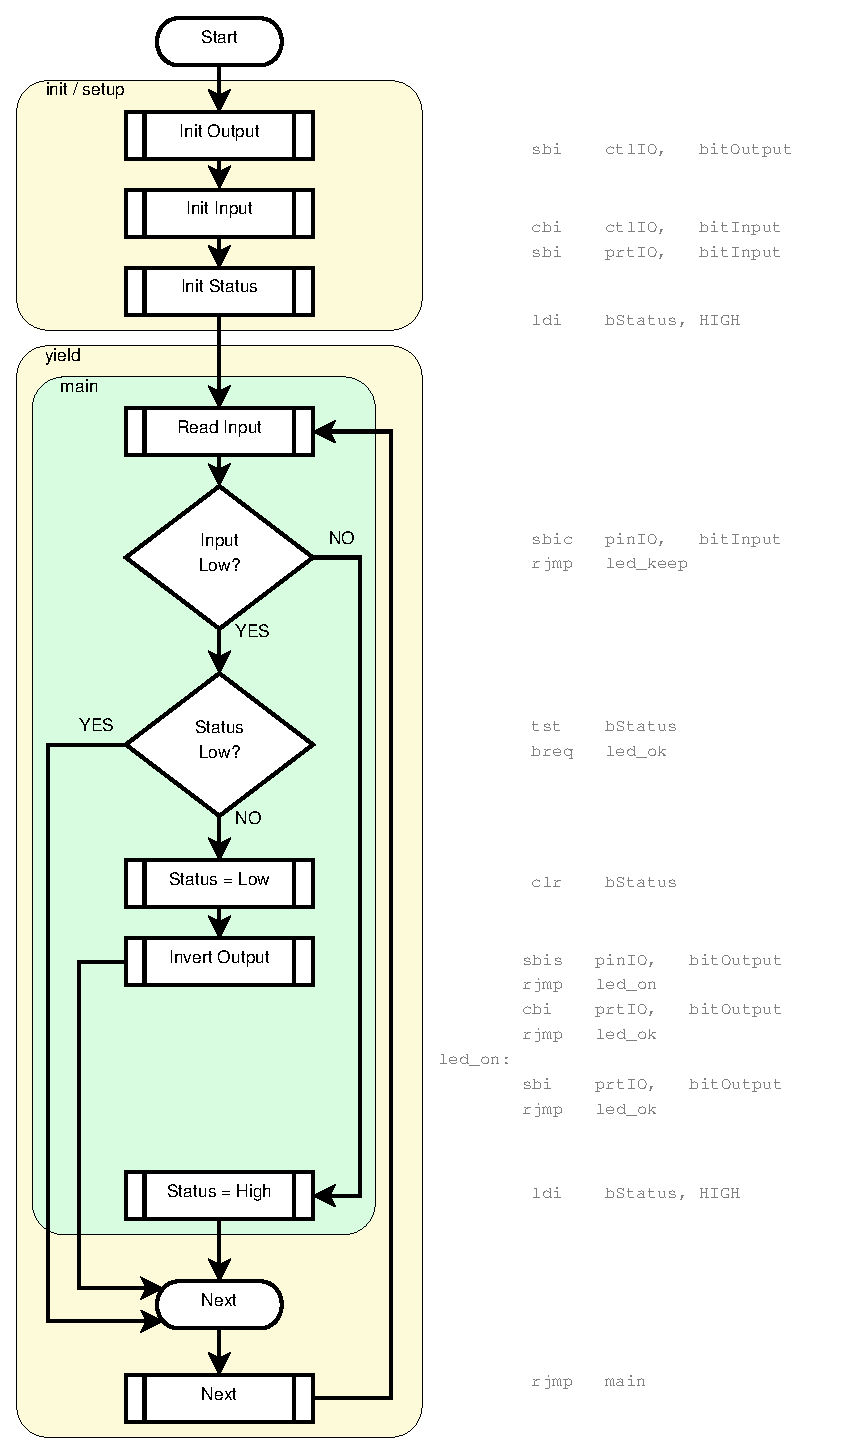
\includegraphics[height=210mm]{LED/S005_stable-decisions+symbols.eps}
  \caption{Stable Decisions - Flow Diagram}
  \label{S005FlowDiagam}
\end{figure}

As you may have found out until now, dealing with the 'human device interface' is the most complicated thing in informatics. It starts with the unbearable slowness of bio entities and does not end with humans expectations against machines. Which means the user is problem number one in software development and for this has to be the main focus! Otherwise your product will not be accepted by those who should pay our wages!

\subsubsection{Slow users}

A living entity presses a button and our device has to react. Our device may ask the input pin about 1.000.000 times per second. A human for example may do a very short pressing of a button in about 0.2 seconds. Which means, our System reads the status 'button pressed' about 200.000 times during our humans action. But what the human expects is:

\begin{center}
Change the light ones as I press (in my view) the button ones!
\end{center}

A problem we will not deal with in this phase of our development is, that electric switches may flicker during status change. Flickery leads to problems because it will generate random additional signals during the action phase. In general this is dealt with by electronically measures. Therefore we simply have to ensure that changing the LEDs status only happens ones per button press action and we will ignore any flickery event by not doing anything about it.

\subsubsection{Fast feedback}

Our feedback device is the light we control. We have no display oder acoustic device to us as feedback but the very same object that goes to be controlled. User feedback therefore simply means to manipulate the status of the light. Even if its cool in movies to do anything without any visible feedback, real living bio entities require 'immediate feedback' for every action. Otherwise they run into problems.


\begin{figure}[htbp]
  \centering
  \includegraphics[width=120mm]{LED/S005_stable-decisions_ideal_signal.png}
  \caption{Stable Decisions - Signal Diagram}
  \label{S005SignalDiagam}
\end{figure}

Figure \ref{S005SignalDiagam} shows the signal we have to expect (idealised). You have to remember, that our micro controller reads the 'LOW' status of the signal 100.000 times or more often. We do not measure time! The natural timing unit in micro controllers is cycles. Read cycles, CPU cycles, sensor cycles. This is important to recognise especially because different clock frequencies and different voltage leads to different physical cycle durations. A program that measures a certain event by 1000 cycles will receive 2000 if the clock is doubled up.

Different clock frequencies lead to different CPU dependent cycles. Different voltage may lead to different sensor cycles, depending on the specification of the sensor in question and the characteristics of the signal to measure. Further, different voltage may lead to different absolute sensor signals, but this is another chapter.

The signal we need to recognise at the moment is the switch from HIGH to LOW and back again. The LOW level will stay for an undefined time / amount of measure cycles. What we have to focus on is the change of the signal!

To deal with this there are only two moments in all this 'endless' button down phase - between 't1' and 't2' - where it is applicable to really change the LEDs status. At the beginning, as the signal changes from HIGH to LOW (t1) or at the end, where the signal changes from LOW to HIGH again (t2).

To give the human who uses our device (the user) immediate feedback about success or failure of his action, we decide to use the first phase (t1) to do all the action. So we have a simple mission: If the signal is LOW now and was HIGH the last time we looked, we change the LEDs state. This satisfies also the endless LOW state of the input signal and the change from LOW to HIGH where we have to do nothing. Not even accidentally! This way, the human feels his request immediately answered, even if he is unable to comprehend on which grade immediately it real is answered.


\subsection{Finding the event}

To find the event the signal has gone to ground, we have to be aware of the status of the signal from the previous query cycle. Which is easy but expensive. We simply use a register to store the previous input status.

We simply have to check if the last seen status was HIGH as log as the current status is LOW. The status accumulator register follows the status of the input signal after being used to query the change event.

If the one moment we are waiting for passes, we invert the LED status. That's all


\subsection{And some modesty}

In respect of things to come, we have to be modest in our style. The 'endless loop' which keeps the micro controller running and waiting without going wild, will be used for some important things:

\begin{itemize}
  \item It mostly contains the main program
  \item It possibly consist of multiple parts
  \item It consist of an undefined amount of functional separate program parts
\end{itemize}

So we have to ensure, to don't make any shortcut back to the 'main' label. As there can only be one Highlander, there can only be one jump back to 'main'. This jump resides at the very end of the main sequence. Like this:

\begin{lstlisting}
main:

  A_begin:
            block     A or goto to end of block A
  A_end:

  B_begin:
            block     B or goto to end of block B
  B_end:

  C_begin:
            block     C or goto to end of block C
  C_end

mein_end:
            finalise
            rjmp      main
\end{lstlisting}

In our flow diagram one part has to reach the next part regardless of how the program is flowing. The rounded rectangle 'next' represents the central point behind our (currently) one part. This is the position where the next program part would follow in the same manner.

